\section{Interpretability}\label{section:interpretability-def}

There is no one formal definition of interpretability and/or explainability in the context of machine learning, and often it is used interchangeably \cite{guidotti2018survey}. Arrieta et al. \cite{arrieta2020explainable} distinguish between the two and define them as:

\begin{definition}[Interpretability]\label{def:interpretability}
Passive characteristic on a model refers to the level of understanding of the models' internal decision process for a human observer.
\end{definition}

\begin{definition}[Explainability]\label{def:explainability}
Active characteristic of a model, associated with the notion of explanation of the action or procedure taken by the model with the intent of clarifying its internal decision process.
\end{definition}

The name of the field Explainable Artificial Intelligence (XAI) refers to the characteristic of a model, but any representation presented to the human (like input attribution) refers to the interpretability of the model. This thesis focuses on the interpretability of CNNs and uses the taxonomy of interpretability as defined in Figure \ref{fig:taxonomy-interpretability} \cite{lipton2018mythos}.

\subsection{Taxonomy of interpretability}\label{section:taxonomy-xai}

\begin{figure}[ht]
    \centering
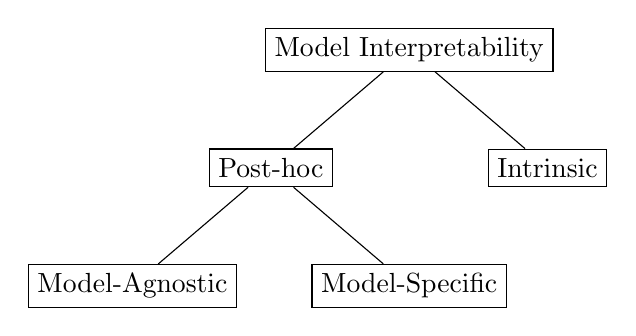
\begin{tikzpicture}[sibling distance=10em,
  every node/.style = {shape=rectangle,
    draw, align=center,
    top color=white, bottom color=white}]]
  \node  {Model Interpretability}
      child { node {Post-hoc}
        child { node {Model-Agnostic} }
        child { node {Model-Specific} } }
      child { node {Intrinsic} };
\end{tikzpicture}
    \caption{Taxonomy of the model interpretability.}
    \label{fig:taxonomy-interpretability}
\end{figure}

There are two major types of models: \textit{white-box models} and \textit{black-box models}. Interpretability of the first type is defined as the \textit{Intrinsic} \cite{biran2017explanation}. This type of interpretability covers all models which have an interpretable internal structure. As an example, the structure of a decision tree is considered interpretable, as well as the internal structure of a shallow neural network. This does not apply to deep neural networks where \textit{post-hoc} interpretability is used. The post-hoc interpretability means that we are trying to explain a prediction of the model without explaining the exact internal mechanism of that model. Because of the complexity of CNNs, post-hoc interpretability is the only way to interpret this kind of model.

\begin{remark}
This is not the only taxonomy of interpretability. The structure of the interpretability can be defined in many ways (either by the purpose, by the method, or by the application).
\end{remark}

\subsubsection*{Model-Agnostic and Model-Specific}

As shown in the taxonomy (see Fig. \ref{fig:taxonomy-interpretability}), post-hoc interpretability is divided into \textit{model-agnostic} and \textit{model-specific} \cite{adadi2018peeking}. The model-agnostic methods are the methods that can be applied to any black-box model without the concern about the internal structure of the model. These methods are usually less precise but because they explain the models' behavior only based on the input and the output. On the other hand, model-specific methods are associated with a particular type of model. The "type" is loosely defined and can refer to the whole domain like CNNs or the specific architecture of CNN. In this thesis, both types of post-hoc interpretability are used.

\subsection{Right to explanation}

The "right to explanation" is a term used by the European Parliament and Council in the General Data Protection Regulation (GDPR) \footnote{Reg (EU) 2016/679 of the European Parliament and of the Council of 27 April 2016 on the protection of natural persons with regard to the processing of personal data and on the free movement of such data, and repealing Dir 95/46/EC (General Data Protection Regulation) 2016.}. This term is often mentioned in regard to XAI methods and requires a data controller to explain how the mechanism reached a decision. This part of the GDPR was created with an intent to prevent using the systems what decision cannot be interpreted by the human (like deep neural networks). The goal is to avoid discrimination and ethical/financial biases in such systems. As an example, we can use the automated credit scoring system. Systems like that are used in the mortgage loan process. It is legally forbidden to discriminate against a person base on a list of characteristics, but that discrimination can be hidden inside a black-box system (even without the knowledge of the creator of that system). If the application is refused by the bank, the applicant can require an explanation of why it was refused. This might help to potentially improve the score before the next application.